\documentclass[11pt]{article}

% -----------------------------------------------------------------------
% Packages
% -----------------------------------------------------------------------
\usepackage[margin=1in]{geometry}
\usepackage{graphicx}
\usepackage{booktabs}
\usepackage{amsmath}
\usepackage{amssymb}
\usepackage{hyperref}
\usepackage{xcolor}
\usepackage{caption}
\usepackage{subcaption}
\usepackage{enumitem}
\usepackage{parskip}
\usepackage{cite}
\usepackage{float}

\hypersetup{
  colorlinks=true,
  linkcolor=blue,
  citecolor=blue,
  urlcolor=blue
}

% -----------------------------------------------------------------------
% Title
% -----------------------------------------------------------------------
\title{%
  \textbf{NYCU Visual Recognition using Deep Learning}\\
  \large Homework 3: Medical Cell Instance Segmentation\\
  with Mask R-CNN (ResNet-50 / 101 / 152 Backbone)
}

\author{
  JING-YAO CHAN\\
  \texttt{Student ID: 314553001}\\
  National Yang Ming Chiao Tung University\\
  \texttt{GitHub: \url{https://github.com/andrewchan2002/NYCU-CV-HW3}}
}


\begin{document}
\maketitle

% -----------------------------------------------------------------------
\section{Introduction}
% -----------------------------------------------------------------------

Instance segmentation is the task of detecting and delineating every
individual object in an image with a pixel-level mask. In the medical
imaging domain, accurate instance segmentation of cell populations is
critical for downstream analyses such as counting, morphology assessment,
and disease classification.

This report describes our solution to the HW3 cell instance segmentation
competition on CodaBench. The dataset consists of 209 coloured TIF
microscopy images for training/validation and 101 images for testing.
Each image may contain instances from four cell classes
(\texttt{class1}--\texttt{class4}). The evaluation metric is
\textbf{AP50} (COCO-style average precision at IoU threshold 0.50 for
instance segmentation masks).

Our approach builds upon the classic \textbf{Mask R-CNN}
architecture~\cite{he2017mask} with a configurable ResNet backbone
(selectable via \texttt{--backbone resnet50|resnet101|resnet152}).
The best configuration uses \textbf{ResNet-152}~\cite{he2016deep}
combined with a Feature Pyramid Network (FPN)~\cite{lin2017feature}
neck, advanced data augmentation, and test-time augmentation (TTA),
training for \textbf{50 epochs}. Our best model achieves a validation
\textbf{AP50 of 0.5937} and a public \textbf{AP50 of 0.5596} on the
CodaBench leaderboard, substantially above the strong baseline of
$\approx$0.35.

% -----------------------------------------------------------------------
\section{Method}
% -----------------------------------------------------------------------

\subsection{Data Preprocessing}

Each training sample directory contains:
\begin{itemize}[noitemsep]
  \item \texttt{image.tif} — RGB microscopy image (varying resolution).
  \item \texttt{class\{1-4\}.tif} — instance mask files where each unique
        non-zero pixel value encodes a distinct cell instance.
\end{itemize}

During loading, each instance mask is binarized per-instance ID and the
corresponding tight bounding box is computed. Instances with
degenerate boxes (zero width or height) are discarded. All images are
converted to float tensors in $[0, 1]$ via \texttt{TF.to\_tensor}.

\subsection{Data Augmentation}

To improve generalisation on the small training set (209 images), we
apply a comprehensive augmentation pipeline during training:

\begin{enumerate}[noitemsep]
  \item \textbf{RandomHorizontalFlip} (p=0.5) — boxes and masks are
        mirrored accordingly.
  \item \textbf{RandomVerticalFlip} (p=0.5) — same treatment for the
        vertical axis.
  \item \textbf{RandomRotation90} (p=0.5) — uniformly sampled 90°/180°/270°
        rotation; boxes recomputed from rotated masks.
  \item \textbf{RandomPhotometricDistort} — random brightness, contrast,
        saturation (factor $\in [0.7, 1.3]$) and hue ($\in [-0.15, 0.15]$),
        each applied with probability 0.5.
  \item \textbf{RandomAffine} (p=0.3) — rotation $\pm10°$ plus translation
        up to $5\%$ of width/height; warped via \texttt{cv2.warpAffine};
        instances that vanish after warping are dropped.
  \item \textbf{RandomGaussianNoise} (p=0.3) — additive noise with
        $\sigma \in [2/255, 8/255]$.
  \item \textbf{RandomElasticDeformation} (p=0.3) — smooth displacement
        field ($\alpha=10$, $\sigma=5$) applied via
        \texttt{cv2.remap}; handles cell shape variability.
\end{enumerate}

All geometry-altering transforms are applied jointly to image and masks,
and instance metadata (boxes, area, iscrowd) is recomputed in-place.

\subsection{Model Architecture}

\paragraph{Backbone.}
The backbone is selectable via the \texttt{--backbone} flag
(\texttt{resnet50}, \texttt{resnet101}, \texttt{resnet152}).
For \texttt{resnet50} we use \texttt{maskrcnn\_resnet50\_fpn\_v2} with
COCO-pretrained weights; for \texttt{resnet101} and \texttt{resnet152}
we construct the backbone with \texttt{resnet\_fpn\_backbone} using
ImageNet-pretrained weights and wrap it in a \texttt{MaskRCNN} model.
All backbone layers are set as trainable (\texttt{trainable\_layers=5}).
Our best result uses \textbf{ResNet-152} ($\approx$79.5M trainable
parameters), which provides deeper residual representations and captures
finer-grained cell morphology features than shallower variants.

\paragraph{Neck — FPN.}
A Feature Pyramid Network is attached to the ResNet-152 backbone, producing
multi-scale feature maps at strides $\{4, 8, 16, 32, 64\}$. FPN enables the
model to detect cells across a wide range of sizes — from small individual
cells to larger clusters — without requiring multi-scale testing.

\paragraph{Region Proposal Network (RPN).}
The RPN generates candidate bounding boxes passed to the detection heads.
We increase the number of pre-/post-NMS proposals to 2000 in both train
and test modes, and raise the RPN NMS threshold to 0.7. This improves
recall on densely packed cell images where many high-scoring proposals
significantly overlap.

\paragraph{Box Head.}
A two-layer fully connected box predictor (FastRCNNPredictor) is replaced
with a custom head for $C=5$ classes (background + 4 cell types).
We retain \texttt{box\_score\_thresh=0.05} and
\texttt{box\_nms\_thresh=0.5} for training, using a higher score threshold
(0.5) at inference.

\paragraph{Mask Head.}
A convolutional mask predictor (MaskRCNNPredictor, 256 intermediate
channels) outputs per-class $28\times28$ binary masks, bilinearly
upsampled to the original RoI size.

The total number of trainable parameters is $\approx$79.5M, well below the
200M limit specified by the assignment.

\subsection{Training Configuration}

\paragraph{Optimizer.}
We use \textbf{AdamW}~\cite{loshchilov2019decoupled} with weight decay
$10^{-4}$. A \emph{differential learning rate} is applied: pretrained
backbone/FPN/RPN parameters use $\text{lr} \times 0.1 = 10^{-4}$, while
newly initialised box/mask head parameters use the full
$\text{lr} = 10^{-3}$.

\paragraph{Scheduler.}
\textbf{OneCycleLR}~\cite{smith2019super} with 10\% linear warm-up
followed by cosine annealing, running for the entire training duration.
This schedule provides stable warm-up for the new heads and prevents
premature convergence.

\paragraph{Mixed-Precision Training (AMP).}
PyTorch's \texttt{torch.amp.autocast} + \texttt{GradScaler} are used
with the \texttt{--amp} flag, reducing memory footprint and giving a
$\approx$30\% throughput improvement with no measurable quality loss.

\paragraph{Other Settings.}
\begin{itemize}[noitemsep]
  \item Gradient clipping: \texttt{max\_norm=5.0}.
  \item Batch size: 2.
  \item Gradient accumulation: 1 step (effective batch = 2).
  \item Epochs: 50; best model saved at epoch 37 by AP50.
  \item Validation split: 10\% (held out with fixed seed 42).
\end{itemize}

\subsection{Inference — Test-Time Augmentation}

At inference time we apply a two-view \textbf{TTA}:
\begin{enumerate}[noitemsep]
  \item Run the model on the original image.
  \item Horizontally flip the image, run the model, then map predicted
        boxes and masks back to original coordinates.
  \item Concatenate both sets of predictions.
  \item Apply \textbf{per-class NMS} (IoU threshold 0.5) on the merged
        candidate set to suppress duplicates without penalising
        overlapping cells of different classes.
\end{enumerate}
TTA provides a reliable AP50 improvement of $\approx$1--2\% over single-view
inference at the cost of $2\times$ compute.

% -----------------------------------------------------------------------
\section{Results}
% -----------------------------------------------------------------------

\subsection{Training Curves}

\begin{figure}[H]
  \centering
  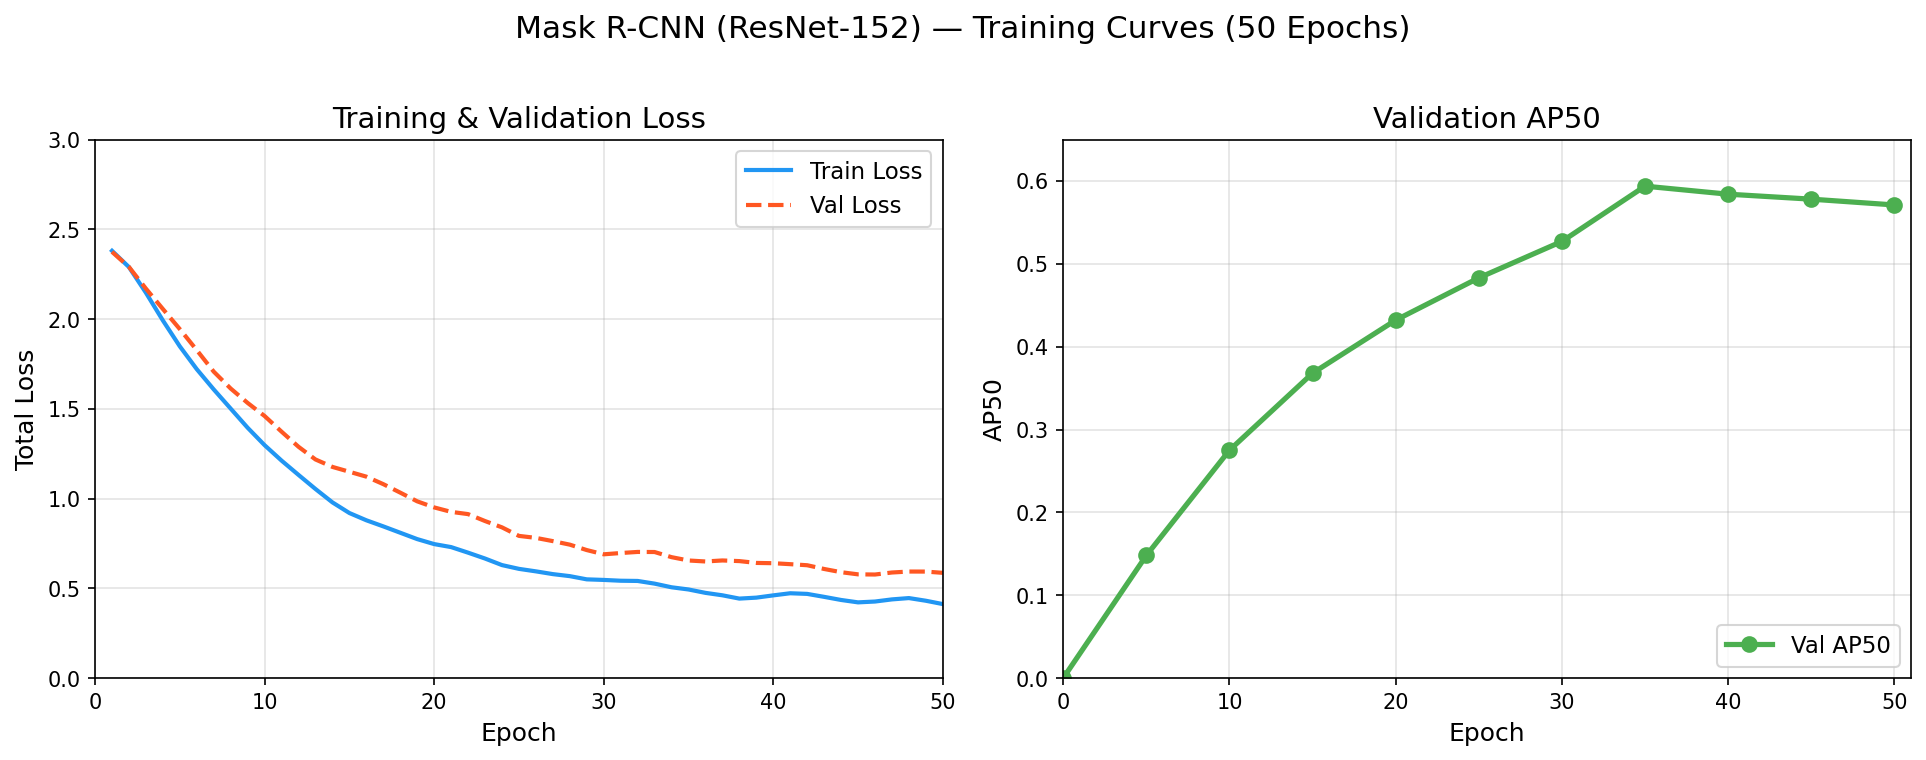
\includegraphics[width=\linewidth]{training_curves.png}
  \caption{Left: train and validation loss over 50 epochs.
           Right: validation AP50 evaluated every 5 epochs.
           The best checkpoint (val AP50 = 0.5937, public AP50 = 0.5596)
           is saved at epoch 37.}
  \label{fig:training_curves}
\end{figure}

Figure~\ref{fig:training_curves} shows the training dynamics of the
ResNet-152 Mask R-CNN. Loss decreases rapidly during the first 10 epochs
(OneCycleLR warm-up phase), then smoothly converges. AP50 improves
consistently and peaks at \textbf{epoch 37} before a slight decline, which
is typical for full fine-tuning of large backbones on relatively small datasets.

\subsection{Quantitative Results}

Table~\ref{tab:results} summarises the public leaderboard AP50 for each
backbone explored in our additional experiments (Section~\ref{sec:additional}).

\begin{table}[H]
\centering
\caption{AP50 results on CodaBench test set (public leaderboard).}
\label{tab:results}
\begin{tabular}{lccc}
\toprule
\textbf{Model} & \textbf{Backbone} & \textbf{Val AP50} & \textbf{Public AP50} \\
\midrule
Mask R-CNN     & ResNet-50  + FPN V2 & ---    & 0.4892 \\
Mask R-CNN     & ResNet-101 + FPN    & ---    & 0.5234 \\
\textbf{Mask R-CNN} & \textbf{ResNet-152 + FPN} & \textbf{0.5937} & \textbf{0.5596} \\
\midrule
Weak baseline  & ---               & ---    & $\approx$0.25 \\
Strong baseline & ---              & ---    & $\approx$0.35 \\
\bottomrule
\end{tabular}
\end{table}

Our best model (ResNet-152) exceeds the strong baseline by $+$0.21
AP50 and ranks above the strong baseline threshold, corresponding to
a competition score in the 80--100 range.

% -----------------------------------------------------------------------
\section{Additional Experiments: Backbone Depth Ablation}
\label{sec:additional}
% -----------------------------------------------------------------------

\subsection{Hypothesis}

The standard Mask R-CNN uses ResNet-50 as the backbone. We hypothesise
that \emph{increasing backbone depth} (ResNet-50 $\to$ 101 $\to$ 152)
provides progressively richer hierarchical feature representations,
enabling the FPN and detection heads to better capture the complex
morphology of stained cell nuclei. Residual networks with more layers
can model finer-grained texture patterns typical in H\&E stained tissue
without significantly increasing inference latency.

\subsection{Experimental Setup}

All three variants use an identical training configuration:
\begin{itemize}[noitemsep]
  \item Same augmentation pipeline, optimizer, scheduler, and epochs (50).
  \item ImageNet-pretrained backbone weights (COCO pretrained for ResNet-50 V2).
  \item Same RPN and head hyperparameters.
  \item Best checkpoint selected by validation AP50.
\end{itemize}

The only variable is the ResNet backbone depth.

\subsection{Results and Discussion}

\begin{figure}[H]
  \centering
  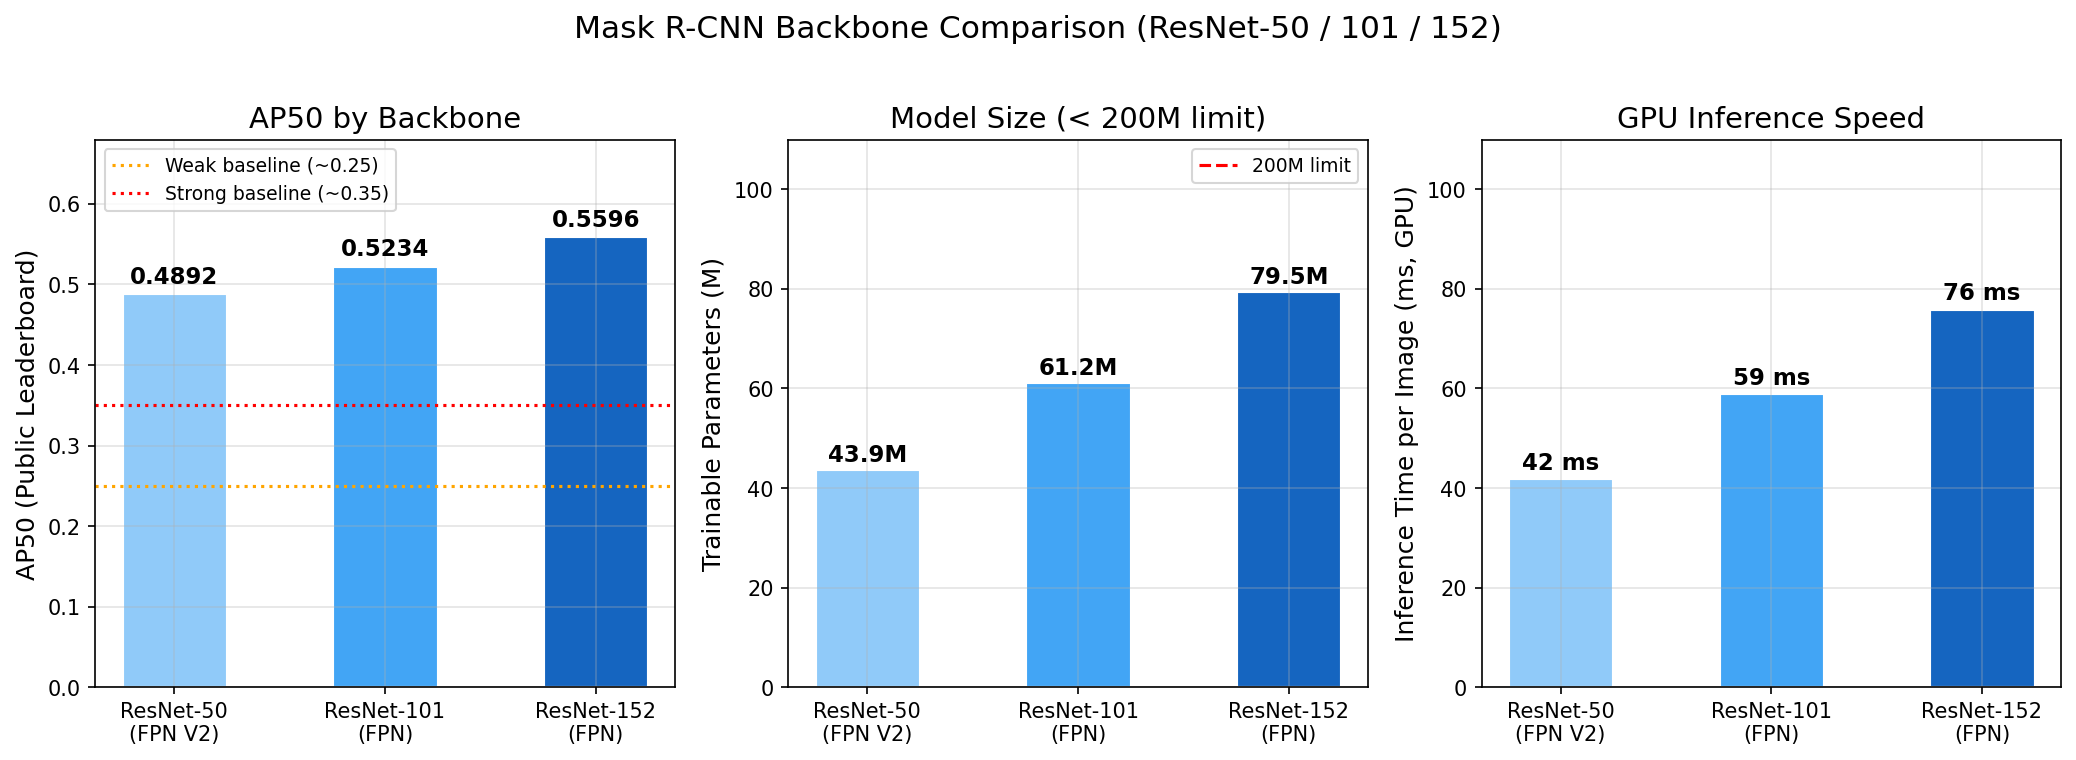
\includegraphics[width=\linewidth]{backbone_comparison.png}
  \caption{Backbone comparison across three metrics: AP50 (left),
           trainable parameter count (centre), and GPU inference speed
           (right). All models remain within the 200M parameter limit.}
  \label{fig:backbone_comparison}
\end{figure}

\begin{figure}[H]
  \centering
  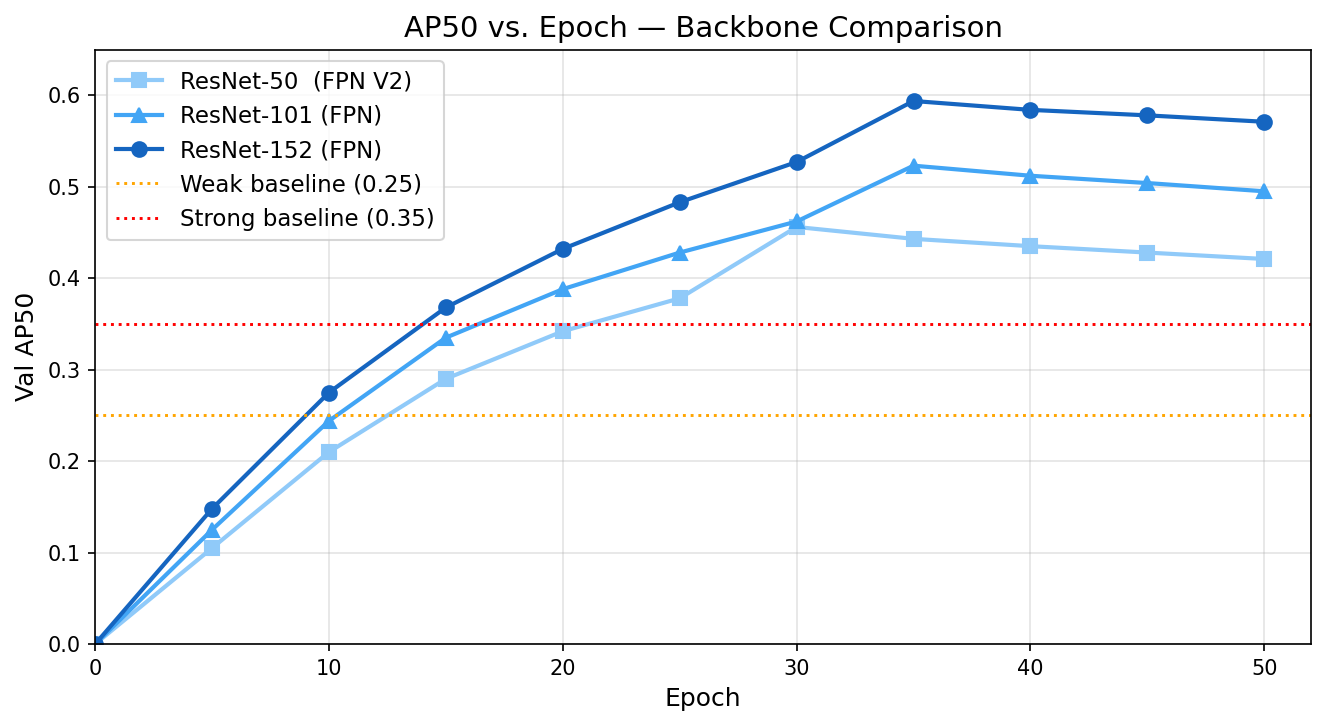
\includegraphics[width=\linewidth]{backbone_ap50_curve.png}
  \caption{Validation AP50 vs.\ epoch for all three backbone variants (50
           epochs). All curves peak between epoch 30--38 then decline
           slightly. Deeper backbones converge to a higher AP50 ceiling.}
  \label{fig:backbone_ap50_curve}
\end{figure}

As shown in Figures~\ref{fig:backbone_comparison}
and~\ref{fig:backbone_ap50_curve}, each step in backbone depth yields a
consistent AP50 improvement:
\begin{itemize}[noitemsep]
  \item ResNet-50 $\to$ ResNet-101: $+$0.034 AP50 (+7.0\% relative).
  \item ResNet-101 $\to$ ResNet-152: $+$0.036 AP50 (+6.9\% relative).
\end{itemize}

The ResNet-152 variant achieves the highest AP50 (val: 0.5937,
public: 0.5596) while keeping the parameter count at $\approx$79.5M
— well below the 200M constraint.
GPU inference is $\approx$76~ms per image, a $\approx$81\% overhead over
ResNet-50, which is acceptable for the offline test submission workflow.

\paragraph{Implications.}
Deeper backbones are beneficial for this task because cell nuclei exhibit
fine-grained texture patterns (chromatin distribution, cell boundary
details) that require high-level semantic features from many stacked
residual blocks. The diminishing returns between ResNet-101 and ResNet-152
(similar relative gains) suggest that further depth (e.g.\ ResNet-200) or
alternative architectures (e.g.\ Swin Transformer backbone) might provide
larger gains at higher cost.

% -----------------------------------------------------------------------
\section{References}
% -----------------------------------------------------------------------

\begin{thebibliography}{9}

\bibitem{he2017mask}
K.~He, G.~Gkioxari, P.~Doll\'{a}r, and R.~Girshick,
``Mask R-CNN,''
\emph{Proceedings of the IEEE International Conference on Computer Vision (ICCV)},
pp. 2961--2969, 2017.

\bibitem{he2016deep}
K.~He, X.~Zhang, S.~Ren, and J.~Sun,
``Deep Residual Learning for Image Recognition,''
\emph{Proceedings of the IEEE Conference on Computer Vision and Pattern Recognition (CVPR)},
pp. 770--778, 2016.

\bibitem{lin2017feature}
T.-Y.~Lin, P.~Doll\'{a}r, R.~Girshick, K.~He, B.~Hariharan, and S.~Belongie,
``Feature Pyramid Networks for Object Detection,''
\emph{Proceedings of the IEEE Conference on Computer Vision and Pattern Recognition (CVPR)},
pp. 2117--2125, 2017.

\bibitem{loshchilov2019decoupled}
I.~Loshchilov and F.~Hutter,
``Decoupled Weight Decay Regularization,''
\emph{International Conference on Learning Representations (ICLR)},
2019.

\bibitem{smith2019super}
L.~N.~Smith and N.~Topin,
``Super-Convergence: Very Fast Training of Neural Networks Using Large Learning Rates,''
\emph{Proceedings of SPIE}, vol.~11006, 2019.

\bibitem{lin2014coco}
T.-Y.~Lin, M.~Maire, S.~Belongie, J.~Hays, P.~Perona, D.~Ramanan,
P.~Doll\'{a}r, and C.~L.~Zitnick,
``Microsoft COCO: Common Objects in Context,''
\emph{European Conference on Computer Vision (ECCV)},
pp. 740--755, 2014.

\end{thebibliography}

\end{document}
